\documentclass[tikz, border=12pt]{standalone}
\usetikzlibrary{positioning}
\begin{document}
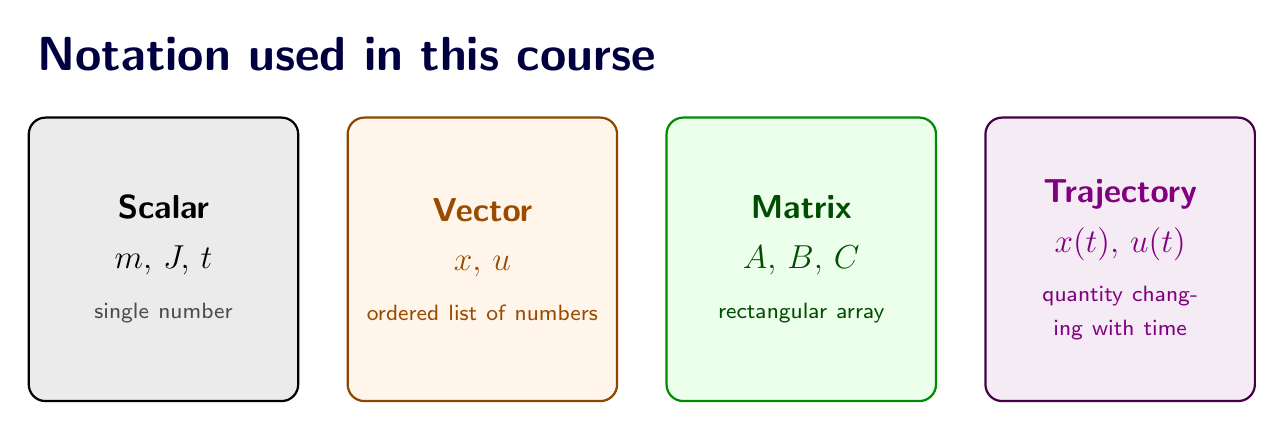
\begin{tikzpicture}[
    font=\sffamily,
    node distance=8mm and 6mm,
    card/.style={rectangle, rounded corners=6pt, draw=#1!55!black, thick,
        fill=#1!8, minimum width=3.4cm, minimum height=3.6cm,
        text width=3.0cm, align=center, inner sep=6pt},
]

\node[font=\sffamily\bfseries\LARGE, text=blue!25!black, anchor=north west]
    (title) at (0,0) {Notation used in this course};

\node[card=black,  below=of title.west, anchor=north west] (scalar)
    {\textcolor{black}{\bfseries\large Scalar}\\[6pt]
     \textcolor{black}{\itshape\large $m,\,J,\,t$}\\[6pt]
     \textcolor{black!70}{\footnotesize single number}};

\node[card=orange, right=of scalar] (vector)
    {\textcolor{orange!60!black}{\bfseries\large Vector}\\[6pt]
     \textcolor{orange!60!black}{\itshape\large $x,\,u$}\\[6pt]
     \textcolor{orange!60!black}{\footnotesize ordered list of numbers}};

\node[card=green, right=of vector] (matrix)
    {\textcolor{green!30!black}{\bfseries\large Matrix}\\[6pt]
     \textcolor{green!30!black}{\itshape\large $A,\,B,\,C$}\\[6pt]
     \textcolor{green!30!black}{\footnotesize rectangular array}};

\node[card=violet, right=of matrix] (traj)
    {\textcolor{violet}{\bfseries\large Trajectory}\\[6pt]
     \textcolor{violet}{\itshape\large $x(t),\,u(t)$}\\[6pt]
     \textcolor{violet}{\footnotesize quantity changing with time}};

\end{tikzpicture}
\end{document}
